%!TEX root = thesis.tex

\chapter{Synopsis}

\begin{figure}
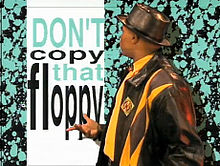
\includegraphics{220px-Dontcopythatfloppy.jpg}
\caption{The ''Disk Protector'' showing the title of the campaign during the rap portion of the video.}
\label{fig:disk_protector}
\end{figure}

Two teenagers, Jenny (played by Marja Allen) and Corey (played by Jimmy Todd), are playing a game on a classroom computer. Corey is exuberantly pushing keys to show the viewer that he is heavily immersed in the game action; Jenny is beating him. Frustrated, he asks for a rematch, but she has an upcoming class and must leave. He decides he will copy the game so that he can play it at home. Upon inserting his blank floppy disk into the Apple Macintosh LC a video pops up on the computer. This video is of a rapper named MC Double Def DP the ''Disk Protector.''

The point of the video is the message that copyright infringement of software will cause the computer and video game industry to lose profit, resulting in halted production of further computer games. \cite{onpi} (The games the video chooses as examples—The Oregon Trail, Tetris, and the Where in the World is Carmen Sandiego? series—were among the most successful and bestselling games of the late-1980s to mid-1990s.)

The rap video portion is interspersed with interviews of artists, writers, programmers and a lawyer. These people are the staff responsible for design of an early version of the game Neverwinter Nights (then an America Online MMORPG) and allows them to explain the issue in greater detail:
\begin{itemize}

    \item Craig Dykstra—America Online—Manager Developer Support
    \item Dave Butler—America Online—Director Platform Software Development
    \item Janet Hunter—America Online—Senior Systems Analyst
    \item Ilene Rosenthal—Software Publishers Association—Attorney
    
\end{itemize}

They explain how games are made, indicating that creating a game can involve 20 to 30 people integrating the various parts, and working on documentation, technical support, and marketing. The point they try to raise is that if sales are low, the authors may decide that the game is unpopular and stop making it.

At the end of the video the DP fades away, leaving Corey and Jenny to decide for themselves whether they will copy the game—they decide against it. Corey, who has some money left over from his summer job, decides that he will buy the game. Jenny agrees and jokes that Corey's game will even come with a manual.

The Wall Street Journal has stated that the film's aesthetic is similar to the TV program Saved By the Bell. It has also highlighted it as an example of classic bubblegum hip-hop with long-run staying power.
\section{Structure of the Thesis}

Apart from the Sysnopsis this Thesis is divided into the following parts:
\begin{description}
  \item[\ref{Criticism}] describes the Reception by the press.
  \item[\ref{popularity_online}] describes the rise of the Video to a meme.
  \item[\ref{sequel}] descibes the Sequel to the video and it's reception.
\end{description}

